\section{データベース設計}

本システムのデータベース設計を ER 図で以下に示す。
\begin{figure}[H]
    \centering
    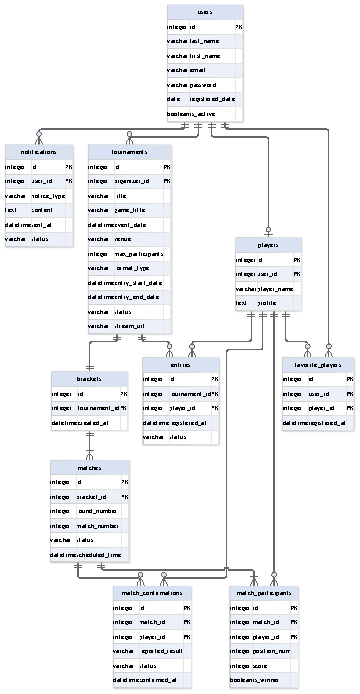
\includegraphics[width=\linewidth, height=0.85\textheight, keepaspectratio]{figures/06/er_diagram_cropped.pdf}
    \caption{データベースER図}
    \label{fig:er_diagram}
\end{figure}

各テーブルの定義を以下の表\ref{tab:users_table}～\ref{tab:notifications_table}に示す。

\noindent\textbf{利用者テーブル（users）}
\begin{table}[H]
    \centering
    \caption{利用者テーブル}
    \label{tab:users_table}
    \begin{tabularx}{\linewidth}{|l|c|c|l|l|X|}
        \hline
        \rowcolor{tableblue}
        \multicolumn{1}{|c|}{カラム名} & \multicolumn{1}{c|}{PK} & \multicolumn{1}{c|}{FK} & \multicolumn{1}{c|}{その他の制約} & \multicolumn{1}{c|}{論理データ型} & \multicolumn{1}{c|}{説明} \\ \hline
        id & 〇 &  & not null, unique & integer & 利用者を一意に識別する番号 \\ \hline
        last\_name &  &  & not null & varchar(50) & 利用者の苗字 \\ \hline
        first\_name &  &  & not null & varchar(50) & 利用者の名前 \\ \hline
        email &  &  & not null, unique & varchar(256) & 利用者のメールアドレス \\ \hline
        password &  &  & not null & varchar(256) & ハッシュ化されたパスワード \\ \hline
        registered\_date &  &  & not null & date & ユーザ登録した日 \\ \hline
        is\_active &  &  & not null & boolean & アカウント有効フラグ（falseで停止） \\ \hline
    \end{tabularx}
\end{table}


\noindent\textbf{選手テーブル（players）}
\begin{table}[H]
    \centering
    \caption{選手テーブル}
    \label{tab:players_table}
    \begin{tabularx}{\linewidth}{|l|c|c|l|l|X|}
        \hline
        \rowcolor{tableblue}
        \multicolumn{1}{|c|}{カラム名} & \multicolumn{1}{c|}{PK} & \multicolumn{1}{c|}{FK} & \multicolumn{1}{c|}{その他の制約} & \multicolumn{1}{c|}{論理データ型} & \multicolumn{1}{c|}{説明} \\ \hline
        player\_id & 〇 &  & not null, unique & integer & 選手を一意に識別する番号 \\ \hline
        player\_name &  &  & not null & varchar(50) & 選手名（大会上で表示されるプレイヤー名） \\ \hline
        user\_id &  & 〇 & not null, unique & integer & 利用者テーブルのID \\ \hline
        profile & & & & text & 公開プロフィール情報（自己紹介・SNS等） \\ \hline
    \end{tabularx}
\end{table}

\noindent\textbf{大会テーブル（tournaments）}
\begin{table}[H]
    \centering
    \caption{大会テーブル}
    \label{tab:tournaments_table}
    \begin{tabularx}{\linewidth}{|l|c|c|l|l|X|}
        \hline
        \rowcolor{tableblue}
        \multicolumn{1}{|c|}{カラム名} & \multicolumn{1}{c|}{PK} & \multicolumn{1}{c|}{FK} & \multicolumn{1}{c|}{その他の制約} & \multicolumn{1}{c|}{論理データ型} & \multicolumn{1}{c|}{説明} \\ \hline
        id & 〇 & & not null, unique & integer & 大会を一意に識別する番号 \\ \hline
        organizer\_id & & 〇 & not null & integer & 主催者の利用者ID（users.id） \\ \hline
        title & & & not null & varchar(200) & 大会名 \\ \hline
        game\_title & & & not null & varchar(100) & 対象ゲーム \\ \hline
        event\_date & & & not null & datetime & 開催日時 \\ \hline
        venue & & & not null & varchar(200) & 開催場所（URLまたは会場名） \\ \hline
        max\_participants & & & not null & integer & 最大参加人数 \\ \hline
        format\_type & & & not null & varchar(30) & 大会形式（シングルエリミネーション等） \\ \hline
        entry\_start\_date & & & not null & datetime & 参加受付開始日時 \\ \hline
        entry\_end\_date & & & not null & datetime & 参加受付終了日時 \\ \hline
        status & & & not null & varchar(20) & 開催状態（予定・開催中・終了済み） \\ \hline
        stream\_url & & & & varchar(500) & 配信URL \\ \hline
    \end{tabularx}
\end{table}

\noindent\textbf{大会参加テーブル（entries）}
\begin{table}[H]
    \centering
    \caption{大会参加テーブル}
    \label{tab:entries_table}
    \begin{tabularx}{\linewidth}{|l|c|c|l|l|X|}
        \hline
        \rowcolor{tableblue}
        \multicolumn{1}{|c|}{カラム名} & \multicolumn{1}{c|}{PK} & \multicolumn{1}{c|}{FK} & \multicolumn{1}{c|}{その他の制約} & \multicolumn{1}{c|}{論理データ型} & \multicolumn{1}{c|}{説明} \\ \hline
        id & 〇 & & not null, unique & integer & 参加情報を一意に識別する番号 \\ \hline
        tournament\_id & & 〇 & not null & integer & 参加する大会のID \\ \hline
        player\_id & & 〇 & not null & integer & 参加する選手のID \\ \hline
        registered\_at & & & not null & datetime & 参加登録日時 \\ \hline
        status & & & not null & varchar(20) & 受付・登録状態（承認待ち・参加確定・キャンセル） \\ \hline
    \end{tabularx}
\end{table}

\noindent\textbf{トーナメントテーブル（brackets）}
\begin{table}[H]
    \centering
    \caption{トーナメントテーブル}
    \label{tab:brackets_table}
    \begin{tabularx}{\linewidth}{|l|c|c|l|l|X|}
        \hline
        \rowcolor{tableblue}
        \multicolumn{1}{|c|}{カラム名} & \multicolumn{1}{c|}{PK} & \multicolumn{1}{c|}{FK} & \multicolumn{1}{c|}{その他の制約} & \multicolumn{1}{c|}{論理データ型} & \multicolumn{1}{c|}{説明} \\ \hline
        id & 〇 & & not null, unique & integer & トーナメント表を一意に識別する番号 \\ \hline
        tournament\_id & & 〇 & not null & integer & 大会ID \\ \hline
        created\_at & & & not null & datetime & トーナメント表作成日時 \\ \hline
    \end{tabularx}
\end{table}

\noindent\textbf{試合テーブル（matches）}
\begin{table}[H]
    \centering
    \caption{試合テーブル}
    \label{tab:matches_table}
    \begin{tabularx}{\linewidth}{|l|c|c|l|l|X|}
        \hline
        \rowcolor{tableblue}
        \multicolumn{1}{|c|}{カラム名} & \multicolumn{1}{c|}{PK} & \multicolumn{1}{c|}{FK} & \multicolumn{1}{c|}{その他の制約} & \multicolumn{1}{c|}{論理データ型} & \multicolumn{1}{c|}{説明} \\ \hline
        id & 〇 & & not null, unique & integer & 試合を一意に識別する番号 \\ \hline
        bracket\_id & & 〇 & not null & integer & トーナメントID \\ \hline
        round\_number & & & not null & integer & ラウンド数（何回戦か） \\ \hline
        match\_number & & & not null & integer & 試合番号 \\ \hline
        status & & & not null & varchar(20) & 試合状態（予定・進行中・完了） \\ \hline
        scheduled\_time & & & & datetime & 試合予定日時 \\ \hline
    \end{tabularx}
\end{table}

\noindent\textbf{試合競技者テーブル（match\_participants）}
\begin{table}[H]
    \centering
    \caption{試合競技者テーブル}
    \label{tab:match_participants_table}
    \begin{tabularx}{\linewidth}{|l|c|c|l|l|X|}
        \hline
        \rowcolor{tableblue}
        \multicolumn{1}{|c|}{カラム名} & \multicolumn{1}{c|}{PK} & \multicolumn{1}{c|}{FK} & \multicolumn{1}{c|}{その他の制約} & \multicolumn{1}{c|}{論理データ型} & \multicolumn{1}{c|}{説明} \\ \hline
        id & 〇 & & not null, unique & integer & 試合と競技者の対応識別番号 \\ \hline
        match\_id & & 〇 & not null & integer & 試合ID \\ \hline
        player\_id & & 〇 & not null & integer & 選手ID \\ \hline
        position\_num & & & not null & integer & 対戦枠（1P枠・2P枠など） \\ \hline
        score & & & & integer & 獲得した得点・ラウンド数 \\ \hline
        is\_winner & & & & boolean & 勝敗（trueで勝利、nullで未定） \\ \hline
    \end{tabularx}
\end{table}

\noindent\textbf{試合結果確認テーブル（match\_confirmations）}
\begin{table}[H]
    \centering
    \caption{試合結果確認テーブル}
    \label{tab:match_confirmations_table}
    \begin{tabularx}{\linewidth}{|l|c|c|l|l|X|}
        \hline
        \rowcolor{tableblue}
        \multicolumn{1}{|c|}{カラム名} & \multicolumn{1}{c|}{PK} & \multicolumn{1}{c|}{FK} & \multicolumn{1}{c|}{その他の制約} & \multicolumn{1}{c|}{論理データ型} & \multicolumn{1}{c|}{説明} \\ \hline
        id & 〇 & & not null, unique & integer & 結果確認を一意に識別する番号 \\ \hline
        match\_id & & 〇 & not null & integer & 試合ID \\ \hline
        player\_id & & 〇 & not null & integer & 結果を入力・確認した選手ID \\ \hline
        reported\_result & & & not null & varchar(255) & 入力された試合結果の内容 \\ \hline
        status & & & not null & varchar(20) & 確認状態（未確認・承認・異議あり） \\ \hline
        confirmed\_at & & & & datetime & 確認完了日時 \\ \hline
    \end{tabularx}
\end{table}

\noindent\textbf{選手お気に入りテーブル（favorite\_players）}
\begin{table}[H]
    \centering
    \caption{選手お気に入りテーブル}
    \label{tab:favorite_players_table}
    \begin{tabularx}{\linewidth}{|l|c|c|l|l|X|}
        \hline
        \rowcolor{tableblue}
        \multicolumn{1}{|c|}{カラム名} & \multicolumn{1}{c|}{PK} & \multicolumn{1}{c|}{FK} & \multicolumn{1}{c|}{その他の制約} & \multicolumn{1}{c|}{論理データ型} & \multicolumn{1}{c|}{説明} \\ \hline
        id & 〇 & & not null, unique & integer & お気に入り登録の識別番号 \\ \hline
        user\_id & & 〇 & not null & integer & 登録した利用者ID \\ \hline
        player\_id & & 〇 & not null & integer & お気に入り対象の選手ID \\ \hline
        registered\_at & & & not null & datetime & 登録日時 \\ \hline
    \end{tabularx}
\end{table}

\noindent\textbf{通知履歴テーブル（notifications）}
\begin{table}[H]
    \centering
    \caption{通知履歴テーブル}
    \label{tab:notifications_table}
    \begin{tabularx}{\linewidth}{|l|c|c|l|l|X|}
        \hline
        \rowcolor{tableblue}
        \multicolumn{1}{|c|}{カラム名} & \multicolumn{1}{c|}{PK} & \multicolumn{1}{c|}{FK} & \multicolumn{1}{c|}{その他の制約} & \multicolumn{1}{c|}{論理データ型} & \multicolumn{1}{c|}{説明} \\ \hline
        id & 〇 & & not null, unique & integer & 通知を一意に識別する番号 \\ \hline
        user\_id & & 〇 & not null & integer & 通知先の利用者ID \\ \hline
        notice\_type & & & not null & varchar(50) & 通知種別（メール・システム等） \\ \hline
        content & & & not null & text & 通知内容のテキスト \\ \hline
        sent\_at & & & not null & datetime & 送信日時 \\ \hline
        status & & & not null & varchar(20) & 送信状態（送信済み・エラー等） \\ \hline
    \end{tabularx}
\end{table}